%! TeX program = lualatex
%! TeX root = main.tex

\def\basedir{/home/theammir/labs/asd/7/res}
\input{/home/theammir/labs/asd/template/template.tex}

\usepackage{amsmath}
\renewcommand{\cosh}{\operatorname{ch}}
\usepackage[hypcap=false]{caption}
\usepackage{graphicx}
\usepackage[colorlinks=true]{hyperref}

\begin{document}
\thetitlepage{7}{ІМ-42}{Туров Андрій Володимирович}{28}

\taskdesc%
Дане натуральне число $n$. Знайти суму перших $n$ членів ряду чисел, заданого рекурентною формулою. Розв'язати задачу трьома способами:
\begin{enumerate}
  \item у програмі використати рекурсивну функцію, яка виконує обчислення і членів ряду, і суми на рекурсивному спуску.
  \item у програмі використати рекурсивну функцію, яка виконує обчислення і членів ряду, і суми на рекурсивному поверненні.
  \item у програмі використати рекурсивну функцію, яка виконує обчислення членів ряду на рекурсивному спуску, а обчислення суми на рекурсивному поверненні.
\end{enumerate}

\taskspec%
\[
\begin{aligned}
  F_1 = 1; F_{i+1} &= F_1 * x^2 \slash \left(4i^2 - 2i\right), \quad i > 0; \\
  \sum_{i=1}^n &= \cosh{x};
\end{aligned}
\]

\codetext{c}

\tasktest%
\begin{figure}[h!]
  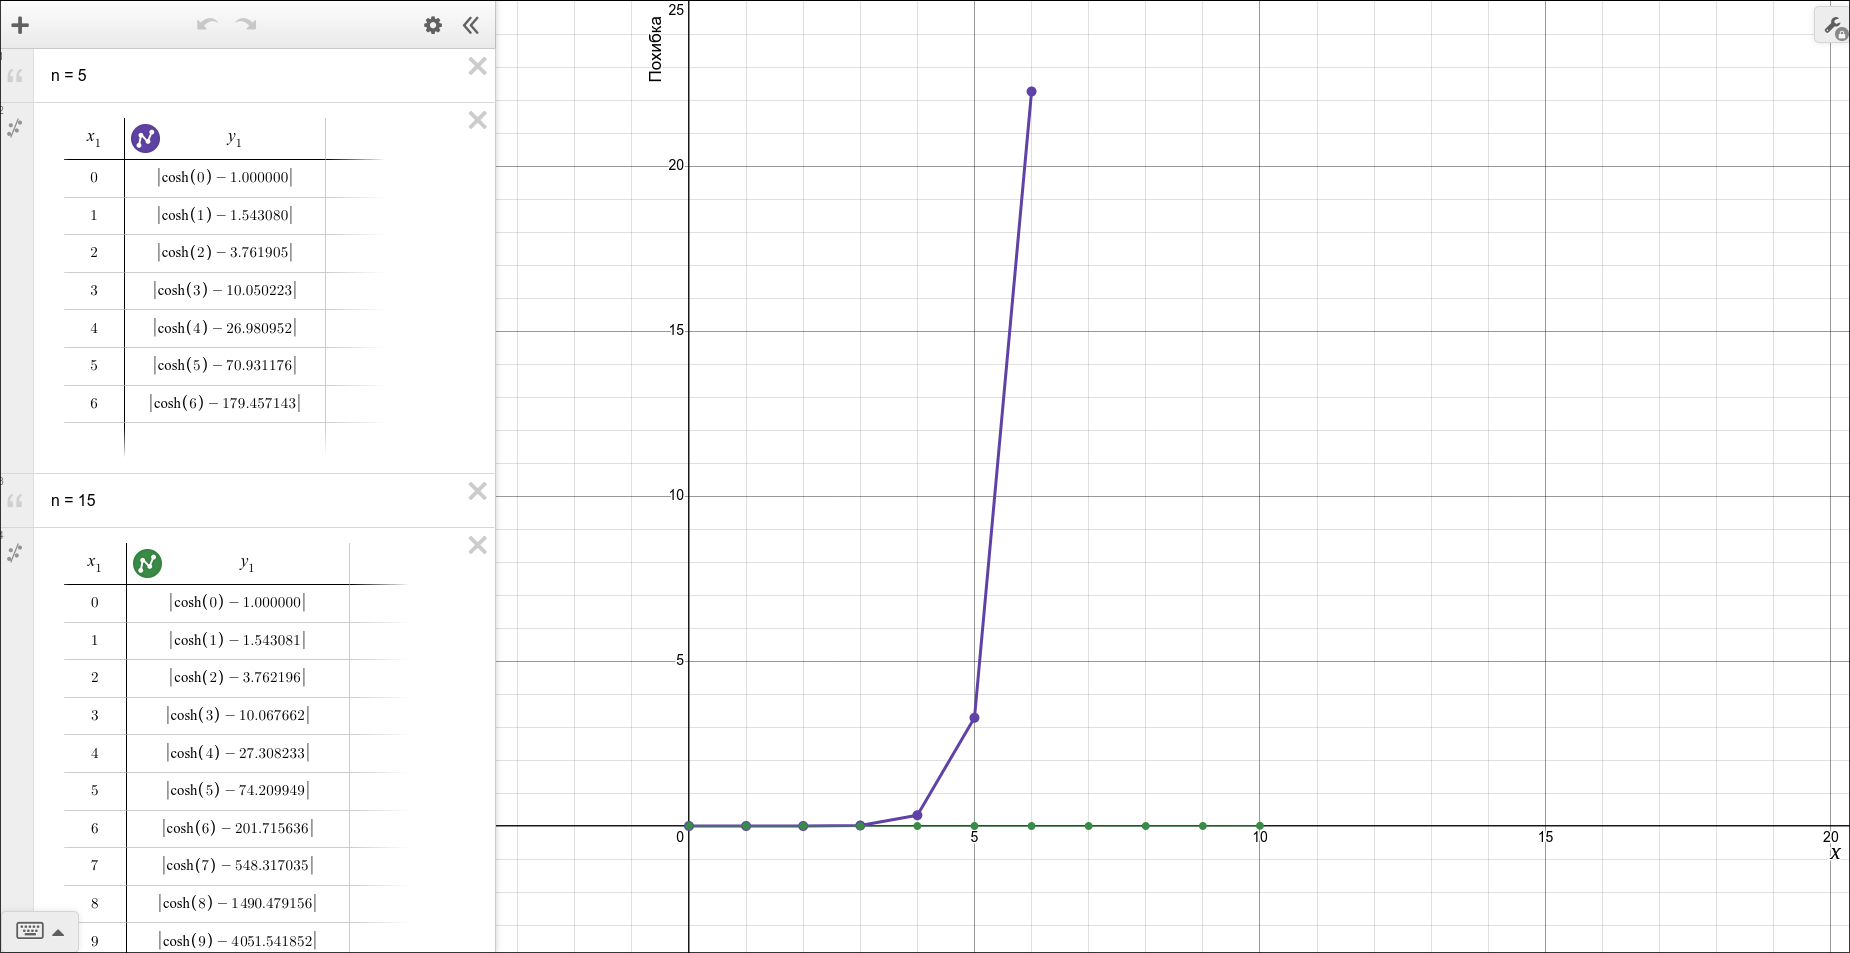
\includegraphics[width=\linewidth]{graph.png}
  \caption{\href{https://www.desmos.com/calculator/ld3qddyify}{Графік} похибки $x$ за різних $n$}
\end{figure}

\begin{minipage}[t]{0.45\linewidth}
  \testcase{./linear 5 1}
  \testcase{./b 5 1}
\end{minipage}
\hfill
\begin{minipage}[t]{0.45\linewidth}
  \testcase{./a 5 1}
  \testcase{./c 5 1}
\end{minipage}

\par
\vspace{3em}

\begin{minipage}[t]{0.45\linewidth}
  \testcase{./a 10 3.1415}
\end{minipage}
\hfill
\begin{minipage}[t]{0.45\linewidth}
  \testcase{./b 10 3.1415}
\end{minipage}

\conclusion%
Навчився використовувати рекурсивні алгоритми для розв'язання задач.
Попрактикувався у написанні рекурсивних функцій, що виконують різні операції на різних етапах виконання.
Ще в \LaTeX{} навчився це все діло оформлювати.

\end{document}

% vim: ts=2: sw=2
